\gene{} instantiates the \ideagene{} framework as a reusable benchmark. It has two parts: \geneexam{} for closed-form lineage understanding and \genearena{} for lineage-grounded idea generation (Figure~\ref{fig:eval}).

\begin{figure}[t]
\centering
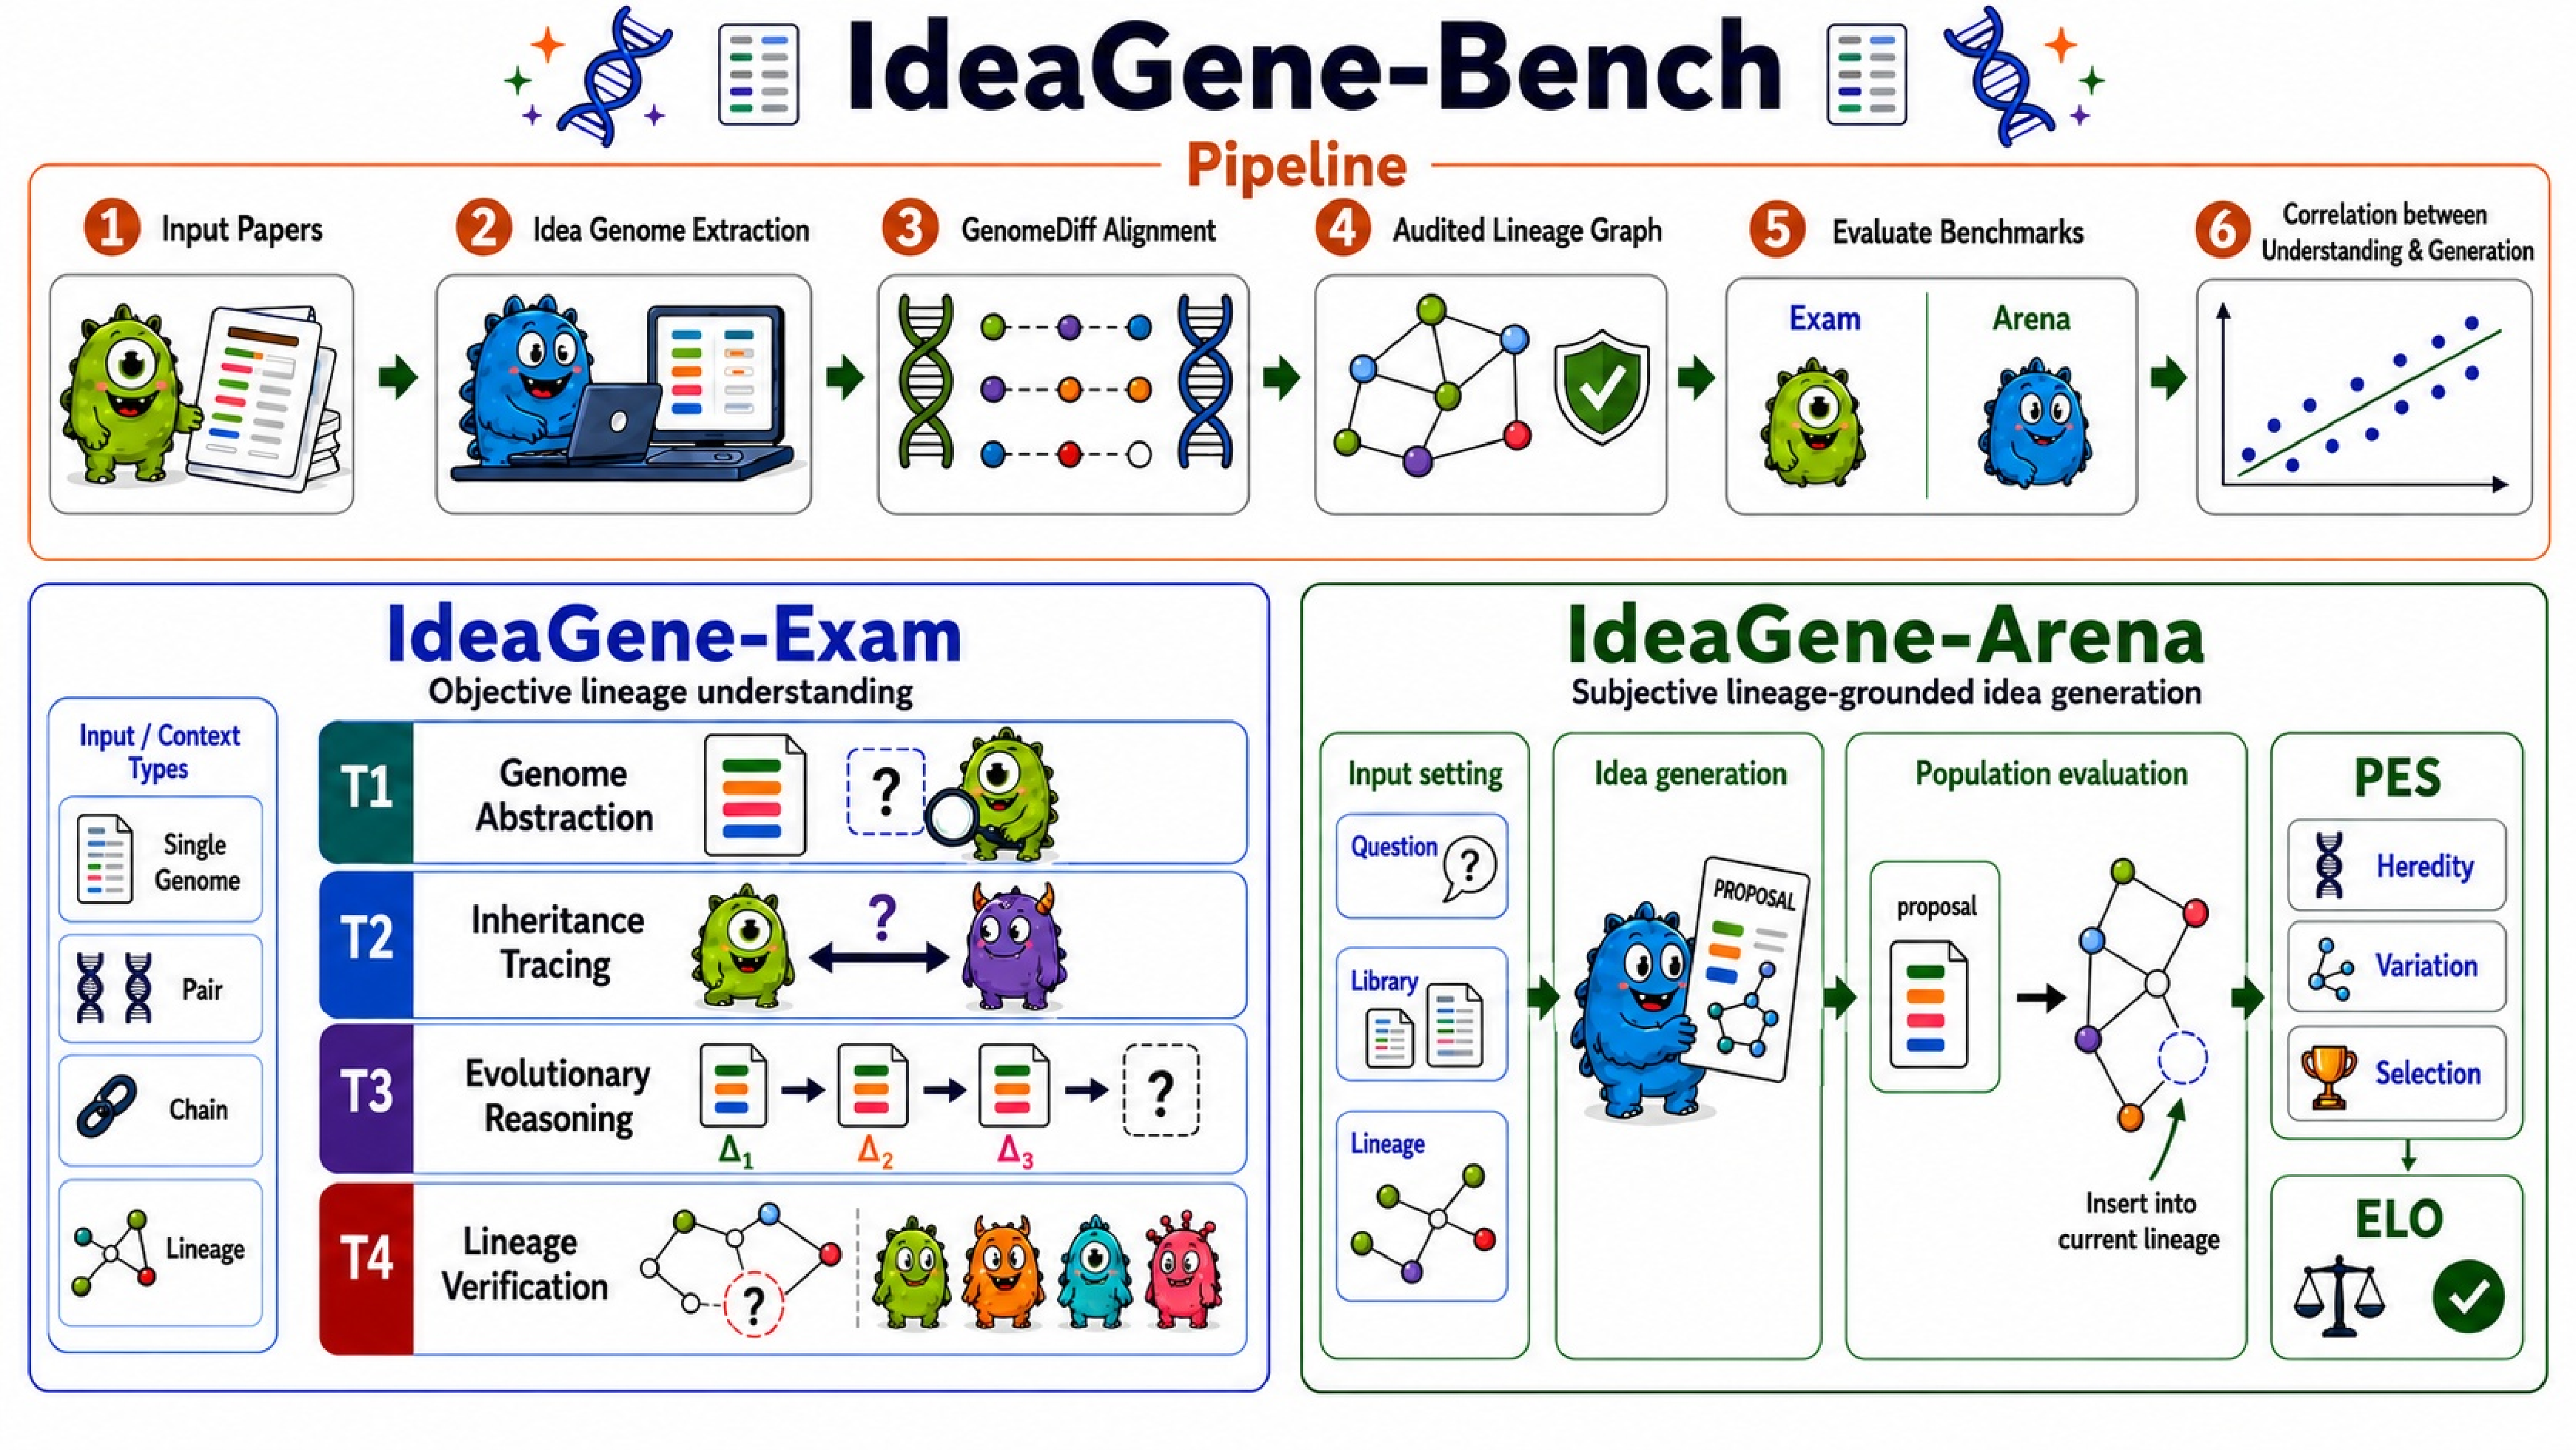
\includegraphics[width=\textwidth]{figures/bench.pdf}
\caption{\textbf{\gene{} evaluation design.} \gene{} converts input papers into a lineage substrate of audited \genome{} objects and \genomediff{} records, then evaluates two complementary capabilities: \geneexam{} for closed-form lineage understanding and \genearena{} for lineage-grounded idea generation. The same substrate supports the correlation between understanding and generation.}
\label{fig:eval}
\end{figure}

\subsection{Data Construction and Quality Assurance}
\label{sec:data_construction}

\gene{} contains 1,961 golden lineage traces across 10 scientific domains---including NLP~\citep{devlin2019bert,radford2019language}, computer vision~\citep{redmon2016yolo,carion2020detr,vit2020}, multimodal learning~\citep{clip2021,llava}, and six additional domains (biology, chemistry, physics, materials, medicine, mathematics). These traces cover 1,085 curated \genome{} objects and 920 pairwise \genomediff{} records. Construction has four stages:

\begin{enumerate}[noitemsep,topsep=2pt,leftmargin=1.2em]
\item \textbf{Seed collection.} Experts nominate landmark and frontier papers in each domain.
\item \textbf{Trace expansion.} We expand candidate predecessors and successors through citation links, semantic search, and domain curation, producing lineage traces of 3--7 papers.
\item \textbf{Genome extraction and diff alignment.} Multi-pass LLM-assisted extraction converts each paper into typed \genome{} objects, which experts then audit. Pairwise \genomediff{} records add object alignment, fate annotation, and driver labels.
\item \textbf{Benchmark-level audit.} Programmatic checks and held-out annotators verify schema validity, answer contracts, temporal consistency, anonymization leakage, and trace coherence.
\end{enumerate}

\paragraph{Quality assurance.} We recruited 50 graduate annotators (master's and doctoral students across computer science, biology, physics, materials science, and other disciplines). They validated three points: \genomediff{} relation labels and role-type assignments during construction, \geneexam{} item difficulty through stratified human solving, and \genearena{} pairwise battles. Construction disagreements were adjudicated by a third annotator. Low human accuracy on \geneexam{} was checked to reflect compositional difficulty rather than label noise, and human judges reached 80\% agreement with the model-judge panel in \genearena{}. Inter-annotator agreement on dynamics labels is 84.7\% before adjudication.

\subsection{\geneexam{}: Lineage Understanding}
\label{sec:gene_exam}

\geneexam{} contains 42 main-challenge task types and 1,029 instances. Each item is
\begin{equation}
\tau=(c,x,\mathcal{A},y,m),
\label{eq:geneexam-item}
\end{equation}
where $c$ is the capability axis, $x$ is anonymized context, $\mathcal{A}$ is the answer space, $y$ is the gold target, and $m$ stores metadata. Scoring uses exact match: every required field must be correct at the same time. A lineage answer is not reliable if it identifies the right parent but assigns the wrong driver or object fate.

\begin{table}[t]
\centering
\small
\caption{\geneexam{} main challenge: 42 task types, 1,029 instances, four capability axes.}
\label{tab:benchmark}
\begin{tabular}{@{}>{\raggedright\arraybackslash}p{4.85cm}@{\;\;}c@{\;\;}c@{\;\;}>{\raggedright\arraybackslash}p{6.35cm}@{}}
\toprule
\textbf{Capability} & \textbf{Tasks} & \textbf{Inst.} & \textbf{Representative tasks} \\
\midrule
T1 Genome Abstraction & 5 & 125 & Identify field type, driver \genome{}, contribution role, or lineage position \\
T2 Inheritance Tracing & 12 & 313 & Reconstruct ordered lineages, align inherited \genome{} objects, match limitations to deltas \\
T3 Evolutionary Reasoning & 17 & 409 & Infer dynamics, driver, object fates, hybrid provenance, or multi-hop changes \\
T4 Lineage Verification & 8 & 182 & Detect intruders, wrong steps, missing links, citation conflicts, or parent mismatch \\
\bottomrule
\end{tabular}
\end{table}

T1 tests whether a model can read a single \genome{}. T2 asks it to trace inheritance across multiple \genome{} objects. T3 requires an explanation of a transition under \genomediff{} criteria. T4 verifies proposed lineage claims and is the closest closed-form analogue to idea generation, because a generated descendant must pass the same parent, coherence, and evidence checks.

\subsection{\genearena{}: Lineage-Grounded Generation}
\label{sec:gene_arena}

\genearena{} evaluates open-ended proposals under controlled information settings. Each instance contains a frontier question, a research domain, an optional paper library, an optional structured lineage, and a scoring rubric. The three settings separate different sources of capability:
\begin{itemize}[noitemsep,topsep=2pt,leftmargin=1.2em]
\item \textbf{Question}: domain and frontier question only; tests parametric ideation.
\item \textbf{Library}: unordered paper summaries; tests paper-centric context use.
\item \textbf{Lineage}: ordered trace with \genome{} objects and \genomediff{} evidence; tests lineage-structured context use.
\end{itemize}

\paragraph{Population-Evolution Score (PES).}
The primary metric is PES, a lineage-conditioned population-insertion score. Rather than judging an idea in isolation, PES evaluates each generated proposal $x$ as a candidate descendant of an ordered lineage $\mathcal{L}$ and a neighboring population $\mathcal{P}$ of related papers or proposals. The judge panel receives a lineage-structured context packet: the frontier question, the ordered lineage, relevant \genome{} objects, \genomediff{} evidence, neighboring population items, and the candidate proposal. PES then decomposes insertion quality into three dimensions that mirror Darwin's conditions for evolution by natural selection~\citep{darwin1859}:

\begin{itemize}[noitemsep,topsep=2pt,leftmargin=1.2em]
\item \textbf{Heredity} ($H$): Relative to $\mathcal{L}$, does the proposal inherit and build on the right parent \genome{} objects? This measures source continuity, mechanism preservation, and limitation-delta coherence under the \genomediff{} evidence.
\item \textbf{Variation} ($V$): Relative to $\mathcal{P}$, does the proposal introduce meaningful novelty? Cosmetic recombination is penalized; substantive mutation, transfer, or new \genome{} objects are rewarded.
\item \textbf{Selection} ($S$): Within the stated lineage population, is the proposal competitively viable? This measures feasibility, fit to the research environment, and whether the proposed work opens productive downstream directions.
\end{itemize}

\noindent Each dimension is scored on a 0--100 scale by a judge panel (3 model judges with position randomization) conditioned on $(\mathcal{L},\mathcal{P})$, and PES is the arithmetic mean:
\begin{equation}
\text{PES}(x \mid \mathcal{L},\mathcal{P}) =
\frac{1}{3}\left(H(x \mid \mathcal{L}) + V(x \mid \mathcal{P}) + S(x \mid \mathcal{L},\mathcal{P})\right).
\label{eq:pes}
\end{equation}
We report PES as the primary metric because it measures lineage-conditioned insertion quality rather than standalone appeal. Pairwise ELO~\citep{elo1978rating}, computed from judge-panel battles under a Bradley--Terry model~\citep{bradley1952rank}, is a complementary preference diagnostic. ELO and PES can diverge: fluency-oriented preferences may favor a polished but lineage-incoherent proposal over a less polished but better-grounded one. We validate PES reliability through inter-judge agreement (Krippendorff's $\alpha = 0.74$~\citep{krippendorff2011alpha}) and human concordance (80\% agreement with the model-judge panel on pairwise rankings).

% \paragraph{Participants.}
% Experiments evaluate direct LLMs, research-agent frameworks, and CLI harnesses under the same task pool and settings. This separates backbone ability from retrieval-heavy agent workflows and from lightweight tool-using scaffolds.
